\documentclass[tikz,border=5pt]{standalone}
\usepackage{tikz}
\usetikzlibrary{arrows.meta,positioning,calc,fit,backgrounds,shapes.geometric,decorations.pathreplacing}
\usepackage{amsmath}
\usepackage{amssymb}
\usepackage{pifont} % proper circled numbers: \ding{192}..\ding{195}
\usepackage{newtxtext,newtxmath} % serif to match NeurIPS body font

\definecolor{coopgreen}{RGB}{40,120,70}
\definecolor{defgray}{RGB}{130,130,130}
\definecolor{msgblue}{RGB}{30,70,150}
\definecolor{rewardorange}{RGB}{200,110,20}
\definecolor{tempyellow}{RGB}{255,243,200}
\definecolor{tempborder}{RGB}{200,170,50}
\definecolor{msgblueligh}{RGB}{220,235,250}
\definecolor{msgborder}{RGB}{70,120,180}

\begin{document}
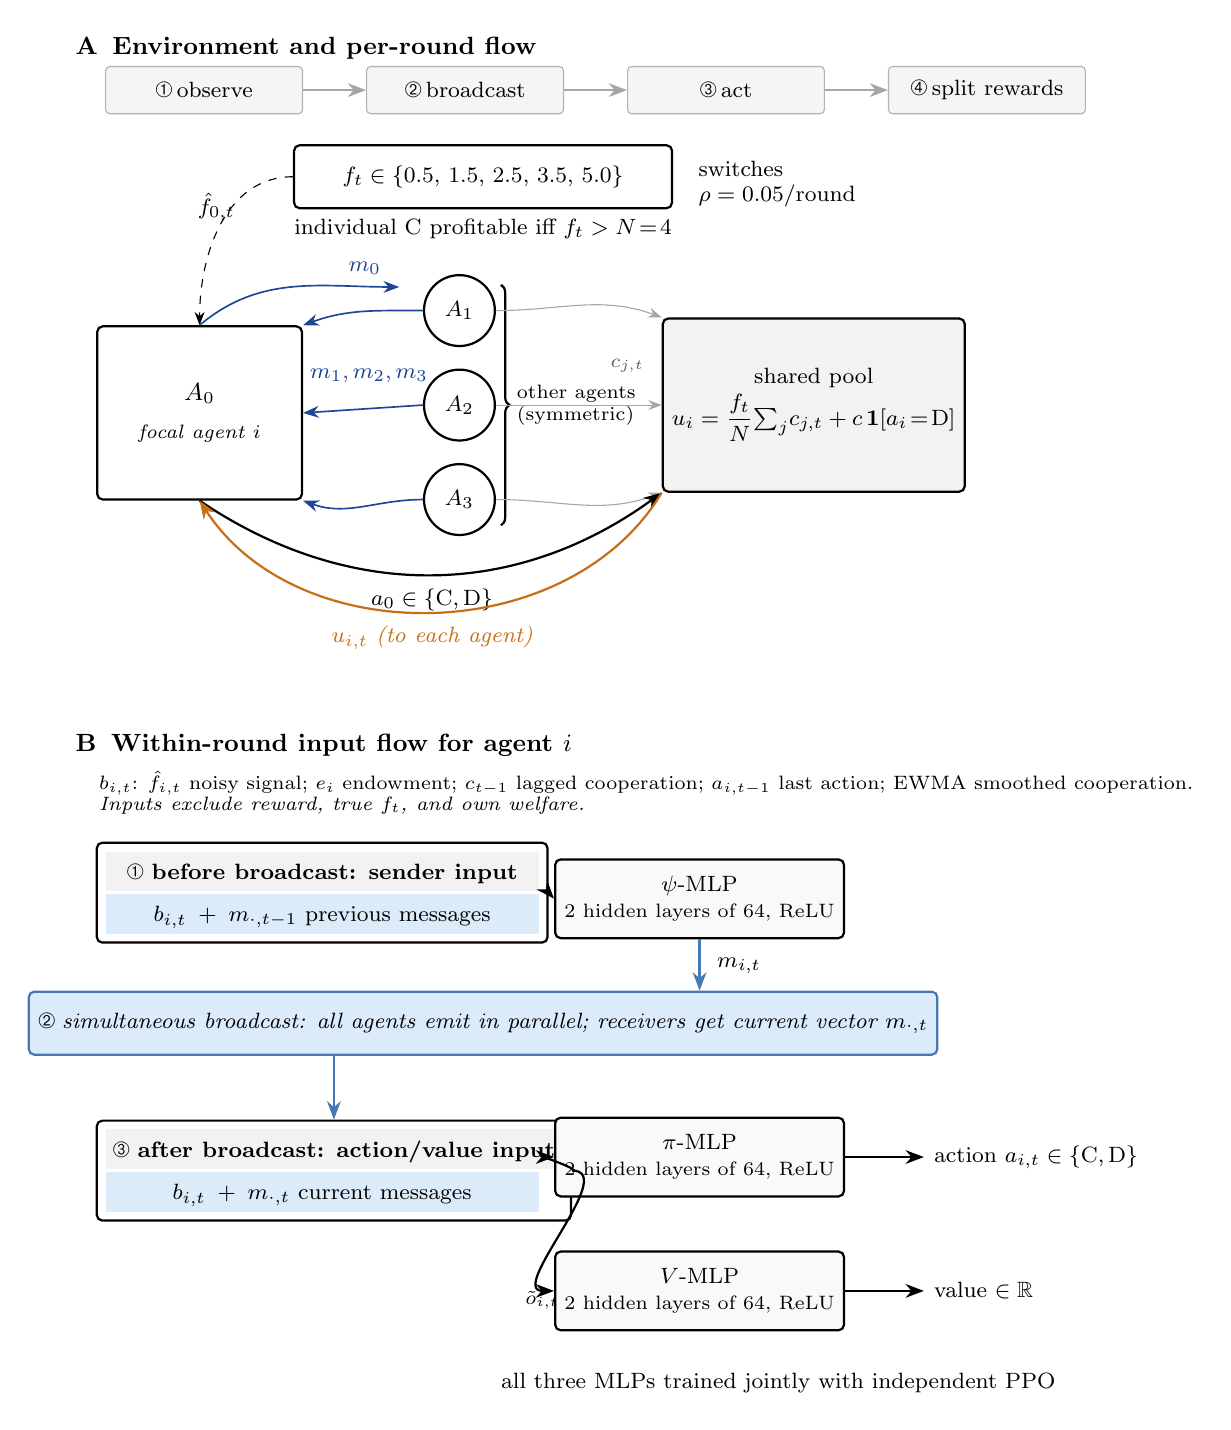
\begin{tikzpicture}[
    font=\footnotesize,
    % Panel A element styles
    agentbox/.style={draw, thick, rounded corners=2pt, minimum width=26mm, minimum height=22mm, align=center, font=\small},
    smallagent/.style={circle, draw, thick, minimum size=9mm, inner sep=0pt, font=\footnotesize},
    poolbox/.style={draw, thick, rounded corners=2pt, fill=gray!10, minimum width=32mm, minimum height=22mm, align=center, font=\footnotesize},
    regimebox/.style={draw, thick, rounded corners=2pt, minimum width=48mm, minimum height=8mm, align=center, font=\footnotesize},
    phasebox/.style={draw=gray!60, fill=gray!8, rounded corners=1.5pt, inner sep=3pt, font=\footnotesize, minimum height=6mm, minimum width=25mm},
    phasearrow/.style={->, >=Stealth, thick, gray!70},
    % Panel B element styles
    obsbundle/.style={draw, thick, rounded corners=2pt, inner sep=0pt},
    obsrow/.style={font=\footnotesize, inner sep=2.5pt, minimum height=5mm, minimum width=45mm, anchor=west, text depth=0pt},
    obshead/.style={font=\footnotesize\bfseries, inner sep=2.5pt, minimum height=5mm, minimum width=45mm, anchor=west, text depth=0pt, fill=gray!10},
    obsrowtemp/.style={obsrow, fill=tempyellow},
    obsrowmsg/.style={obsrow, fill=msgblueligh},
    mlp/.style={draw, thick, fill=gray!5, minimum width=22mm, minimum height=10mm, rounded corners=2pt, align=center, font=\footnotesize},
    head/.style={draw, rounded corners=1pt, minimum width=16mm, minimum height=7mm, font=\footnotesize, inner sep=2pt, align=center},
    % arrows
    flow/.style={->, >=Stealth, thick},
    thinflow/.style={->, >=Stealth, semithick},
    msgflow/.style={->, >=Stealth, semithick, msgblue},
    actflow/.style={->, >=Stealth, thick},
    actflowthin/.style={->, >=Stealth, thin, gray!70},
    rewflow/.style={->, >=Stealth, thick, rewardorange},
    regarrow/.style={->, >=Stealth, dashed, thin},
]

% ============================================================
% PANEL A: ENVIRONMENT AND PER-ROUND FLOW
% ============================================================

\begin{scope}[local bounding box=panelA]

% Panel label
\node[font=\bfseries\small, anchor=north west] at (-0.3,6.8) {A\, Environment and per-round flow};

% Round-sequence workflow strip: wider boxes, longer connecting arrows, spans full panel width
\node[phasebox, anchor=west] (ph1) at (0.2,6.0) {\ding{192}\,observe};
\node[phasebox, right=8mm of ph1] (ph2) {\ding{193}\,broadcast};
\node[phasebox, right=8mm of ph2] (ph3) {\ding{194}\,act};
\node[phasebox, right=8mm of ph3] (ph4) {\ding{195}\,split rewards};
\draw[phasearrow] (ph1.east) -- (ph2.west);
\draw[phasearrow] (ph2.east) -- (ph3.west);
\draw[phasearrow] (ph3.east) -- (ph4.west);

% Regime box (top-center)
\node[regimebox] (regime) at (5.0,4.9) {$f_t \in \{0.5,\,1.5,\,2.5,\,3.5,\,5.0\}$};
\node[anchor=west] at ($(regime.east)+(2mm,1mm)$) {switches};
\node[anchor=west] at ($(regime.east)+(2mm,-2.5mm)$) {$\rho=0.05$/round};

% Strategic threshold hint below regime box
\node[anchor=north, align=center] at (regime.south) {individual $\mathrm{C}$ profitable iff $f_t > N\!=\!4$};

% --- Focal agent A_0 on the left (two-line label: "A_0" + italic subtitle, both inside the box) ---
\node[agentbox, align=center] (a0) at (1.4, 1.9) {$A_0$\\[1mm] {\scriptsize\itshape focal agent $i$}};

% --- Three other agents in the center as stacked small circles ---
\node[smallagent] (a1) at (4.7, 3.2) {$A_1$};
\node[smallagent] (a2) at (4.7, 2.0) {$A_2$};
\node[smallagent] (a3) at (4.7, 0.8) {$A_3$};

% Brace + label for the "other agents (symmetric)" group
\draw[decorate, decoration={brace, amplitude=3pt}, thick]
    ($(a1.north east)+(2mm,0)$) -- ($(a3.south east)+(2mm,0)$)
    node[midway, right=2pt, font=\scriptsize, align=left] {other agents\\(symmetric)};

% --- Pool on the far right, with payoff formula inside ---
\node[poolbox] (pool) at (9.2, 2.0) {shared pool\\[0.5mm] $u_i = \dfrac{f_t}{N}\!\sum_{j}\! c_{j,t} + c\,\mathbf{1}[a_i\!=\!\mathrm{D}]$};

% --- Arrows ---

% 1) Regime -> A_0 (noisy private signal, dashed)
\draw[regarrow] (regime.west) to[out=180, in=90]
    node[pos=0.55, above=0.5mm, font=\footnotesize] {$\hat f_{0,t}$}
    (a0.north);

% 2) m_1, m_2, m_3 -> A_0 (blue, from each small circle into A_0's east side)
\draw[msgflow] (a1.west) to[out=180, in=20] (a0.north east);
\draw[msgflow] (a2.west) -- (a0.east);
\draw[msgflow] (a3.west) to[out=180, in=-20] (a0.south east);
\node[font=\footnotesize, msgblue, anchor=south, align=center] at ($(a0.east)!0.55!(a2.west)+(0,2mm)$) {$m_1,m_2,m_3$};

% 3) A_0 -> others (outgoing message m_0)
\draw[msgflow] (a0.north) to[out=40, in=180]
    node[pos=0.85, above=0.2mm, font=\footnotesize, msgblue] {$m_0$}
    ($(a1.west)+(-3mm,3mm)$);

% 4) Contributions (thin gray) from the three other agents to pool --- to show they all contribute c_{j,t}
\draw[actflowthin] (a1.east) to[out=0, in=160] (pool.north west);
\draw[actflowthin] (a2.east) -- (pool.west);
\draw[actflowthin] (a3.east) to[out=0, in=200] (pool.south west);
\node[font=\scriptsize, gray!70!black, anchor=east] at ($(pool.west)+(-1mm,5mm)$) {$c_{j,t}$};

% 5) A_0 -> pool (focal-agent action, thick black) --- below, clearing the agent stack
\draw[actflow] (a0.south) to[bend right=35]
    node[pos=0.5, below=0.5mm, font=\footnotesize, align=center] {$a_0 \in \{\mathrm{C},\mathrm{D}\}$}
    (pool.south west);

% 6) Pool -> A_0 (reward, deeper bend below) --- orange
\draw[rewflow] (pool.south west) to[bend left=58]
    node[pos=0.5, below=0.5mm, font=\footnotesize, rewardorange, align=center] {$u_{i,t}$ \emph{(to each agent)}}
    (a0.south);

\end{scope}

% ============================================================
% PANEL B: AGENT OBSERVATION AND ARCHITECTURE
% Stacked BELOW Panel A.
% ============================================================

\begin{scope}[local bounding box=panelB, yshift=-9.5cm]

% Panel label and compact observation key
\node[font=\bfseries\small, anchor=north west] at (-0.3,7.45) {B\, Within-round input flow for agent $i$};
\node[font=\scriptsize, anchor=north west] at (0.0,6.98)
      {$b_{i,t}$: $\hat f_{i,t}$ noisy signal; $e_i$ endowment; $c_{t-1}$ lagged cooperation; $a_{i,t-1}$ last action; EWMA smoothed cooperation.};
\node[font=\scriptsize\itshape, anchor=north west] at (0.0,6.65)
      {Inputs exclude reward, true $f_t$, and own welfare.};

% ====================================================================
% STAGE 1: pre-broadcast input  ->  psi-MLP  ->  emits m_{i,t}
% ====================================================================

% Pre-broadcast input box. The base state is defined once above; this box
% highlights that sender emission uses previous-round messages.
\node[obshead, minimum width=55mm] (prehead) at (0.2, 5.58) {\ding{192}\;before broadcast: sender input};
\node[obsrowmsg, minimum width=55mm, below=0.3mm of prehead.south west, anchor=north west] (prerow1)
    {$b_{i,t}\;+\;m_{\cdot,t-1}$ previous messages};
\node[obsbundle, fit=(prehead)(prerow1), inner xsep=3pt, inner ysep=3pt] (prebox) {};

% psi-MLP to the right of the pre-box
\node[mlp, minimum width=24mm, minimum height=10mm] (psimlp) at (7.75, 5.23) {$\psi$-MLP\\{\scriptsize 2 hidden layers of 64, ReLU}};

% Arrow: whole pre-bundle feeds psi
\draw[flow] (prebox.east) -- (psimlp.west);

% ====================================================================
% BROADCAST BUS: simultaneous emission from all agents
% ====================================================================
\node[draw, thick, rounded corners=2pt, fill=msgblueligh, draw=msgborder,
      minimum width=100mm, minimum height=8mm, align=center, font=\footnotesize\itshape]
      (bbus) at (5.0, 3.65) {\ding{193}\;simultaneous broadcast: all agents emit in parallel; receivers get current vector $m_{\cdot,t}$};

% psi output: m_{i,t}
\coordinate (bus_in) at (bbus.north -| psimlp.south);
\node[font=\footnotesize, anchor=west] at ($(psimlp.south)!0.52!(bus_in)+(1mm,0)$) {$m_{i,t}$};

% Arrow: own message drops directly from the sender head into the broadcast bus.
\draw[->, >=Stealth, thick, msgborder, rounded corners=3pt]
    (psimlp.south) -- (bus_in);

% ====================================================================
% STAGE 2: post-broadcast input  ->  pi-MLP and V-MLP
% ====================================================================

% Post-broadcast input box. The action/value heads use the same base state,
% now paired with current-round messages.
\node[obshead, minimum width=55mm] (posthead) at (0.2, 2.05) {\ding{194}\;after broadcast: action/value input};
\node[obsrowmsg, minimum width=55mm, below=0.3mm of posthead.south west, anchor=north west] (postrow1)
    {$b_{i,t}\;+\;m_{\cdot,t}$ current messages};
\node[obsbundle, fit=(posthead)(postrow1), inner xsep=3pt, inner ysep=3pt] (postbox) {};

% Arrow: the broadcast bus delivers current messages to the post-broadcast input.
\coordinate (bus_out) at (bbus.south -| postbox.north);
\draw[->, >=Stealth, thick, msgborder, rounded corners=3pt]
    (bus_out) -- (postbox.north);

% pi-MLP and V-MLP to the right of the post-box
\node[mlp, minimum width=24mm, minimum height=10mm] (pimlp) at (7.75, 1.95) {$\pi$-MLP\\{\scriptsize 2 hidden layers of 64, ReLU}};
\node[mlp, minimum width=24mm, minimum height=10mm] (vmlp) at (7.75, 0.25) {$V$-MLP\\{\scriptsize 2 hidden layers of 64, ReLU}};

% Arrows: whole post-bundle feeds pi and V (with tilde-o on V's arrow)
\draw[flow] (postbox.east) to[out=0, in=180] (pimlp.west);
\draw[flow] (postbox.east) to[out=0, in=180]
    node[pos=0.8, below=0.3mm, font=\scriptsize] {$\tilde o_{i,t}$}
    (vmlp.west);

% Outputs
\draw[flow] (pimlp.east) -- ++(10mm, 0) node[anchor=west, font=\footnotesize] {action $a_{i,t} \in \{\mathrm{C},\mathrm{D}\}$};
\draw[flow] (vmlp.east) -- ++(10mm, 0) node[anchor=west, font=\footnotesize] {value $\in \mathbb{R}$};

% Training annotation
\node[font=\footnotesize, anchor=north] at ($(vmlp.south)+(10mm,-4mm)$) {all three MLPs trained jointly with independent PPO};

\end{scope}

\end{tikzpicture}
\end{document}
